
% use pdflatex -shell-escape slides.tex to compile
\documentclass[10pt]{beamer}
\usetheme[
%%% options passed to the outer theme
%    shownavsym          % show the navigation symbols
  ]{AAUsimple}
  
% If you want to change the colors of the various elements in the theme, edit and uncomment the following lines
% Change the bar and sidebar colors:
%\setbeamercolor{AAUsimple}{fg=red!20,bg=red}
%\setbeamercolor{sidebar}{bg=red!20}
% Change the color of the structural elements:
%\setbeamercolor{structure}{fg=red}
% Change the frame title text color:
%\setbeamercolor{frametitle}{fg=blue}
% Change the normal text color background:
%\setbeamercolor{normal text}{fg=black,bg=gray!10}
% ... and you can of course change a lot more - see the beamer user
% manual.
\usepackage{animate}
\usepackage{epstopdf}
\usepackage{movie15}
\usepackage[utf8]{inputenc}
\usepackage[english]{babel}
\usepackage[T1]{fontenc}
% Or whatever. Note that the encoding and the font should match. If T1
% does not look nice, try deleting the line with the fontenc.
\usepackage{helvet}
\usepackage[helvet]{sfmath}

% For math font script
\usepackage[mathscr]{euscript}

\usepackage{color, xcolor}
\usepackage{tikz}
% tikz setup for descendant robot motion figure 
\usetikzlibrary{positioning,chains,fit,shapes,calc}
\usetikzlibrary{arrows,shadows,trees}
\tikzset{
  basic/.style  = {draw, text width=2cm, drop shadow, font=\sffamily, rectangle},
  root/.style   = {basic, rounded corners=2pt, thin, align=center,
                   fill=red!30},
  level 2/.style = {basic, rounded corners=6pt, thin,align=center, fill=orange!30,
                   text width=8em},
  level 3/.style = {basic, thin, align=left, fill=pink!60, text width=8em}
}
% tikz setup for lattice graph
\usepackage{pgf}
\usetikzlibrary{automata}
\usepackage{hyperref}
\hypersetup{pdfpagemode=FullScreen}
\usepackage{ifthen}
\usepackage{animate}

% tikz animation
\usetikzlibrary{arrows,decorations.pathmorphing,through,backgrounds,positioning,fit,petri}
\usetikzlibrary{shapes.multipart}
\usetikzlibrary{decorations.pathreplacing}

\usepackage[tikz]{bclogo}

\newcommand{\id}{{\rm id}}
\newcommand{\edge}[3]{{#1}\overset{#2}{\longrightarrow}{#3}}
\renewcommand{\L}{{\Lambda}}
% colored hyperlinks
\newcommand{\chref}[2]{%
  \href{#1}{{\usebeamercolor[bg]{AAUsimple}#2}}%
}

\title{Decentralized Formation of Arbitrary Multi-Robot Lattices}

%\subtitle{v.\ 1.0.0}  % could also be a conference name
%\date{\today}
\author{
  \underline{Yang Song}, Jason M. O'Kane\\
  \href{mailto:song24@email.sc.edu}{{\tt song24@email.sc.edu} \\
  \href{mailto:jokane@cse.sc.edu}{\tt jokane@cse.sc.edu}}
}

% - Give the names in the same order as they appear in the paper.
% - Use the \inst{?} command only if the authors have different
%   affiliation. See the beamer manual for an example

\institute[
%  {\includegraphics[scale=0.2]{aau_segl}}\\ %insert a company, department or university logo
  Dept.\ of Computer Science and Engineering\\
  University of South Carolina
] % optional - is placed in the bottom of the sidebar on every slide
{% is placed on the bottom of the title page
  Dept. of Computer Science and Engineering\\
  University of South Carolina
  
  %there must be an empty line above this line - otherwise some unwanted space is added between the university and the country (I do not know why;( )
}

% specify a logo on the titlepage (you can specify additional logos an include them in 
% institute command below
\pgfdeclareimage[height=1.5cm]{titlepagelogo}{sc_logo.pdf}%{aau_logo_new.pdf} % placed on the title page
%\pgfdeclareimage[height=1.5cm]{titlepagelogo2}{aau_logo_new.pdf} % placed on the title page
\titlegraphic{% is placed on the bottom of the title page
  \pgfuseimage{titlepagelogo}
%  \hspace{1cm}\pgfuseimage{titlepagelogo2}
}

\definecolor{scred}{RGB}{115,0,10}% dark red 
\definecolor{myblue}{RGB}{80,80,160}
\definecolor{mygreen}{RGB}{80,160,80}

\begin{document}
% the titlepage
\begin{frame}[plain] % the plain option removes the sidebar and header from the title page
  \titlepage
\end{frame}
%%%%%%%%%%%%%%%%
% TOC
% \begin{frame}{Agenda}{}
% \tableofcontents
% \end{frame}
%%%%%%%%%%%%%%%%

\section{Introduction}
\begin{frame}{Related Work}{}
    \begin{columns}[T] % align columns
      \begin{column}{.45\textwidth}
        \small{Virtual Force}
        \begin{figure}
          \centering
          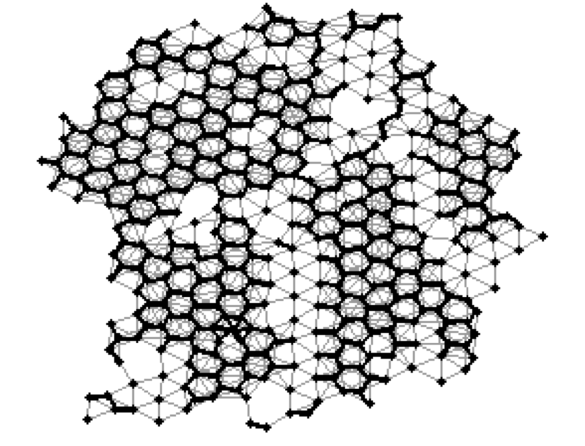
\includegraphics[height=1in]{figs/james.png}
        \end{figure}
        \footnotesize{S. Prabhu, W Li, J. McLurkin, 2012}
      \end{column}%
      \begin{column}{.45\textwidth}
        \small{Task Assignment}
        \begin{center}
        \animategraphics[height=1in,autoplay]{12}{figs/liu_}{0}{18}   
        \end{center}
        \footnotesize{ Lantao Liu and Dylan Shell, 2012}
      \end{column}%
    \end{columns}
    \begin{figure}
      \centering
      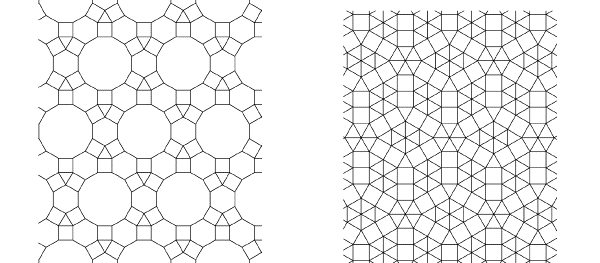
\includegraphics[height=1in]{figs/tessellation.png}
    \end{figure}
\end{frame}

\begin{frame}{Contribution}{}
\begin{block}{}
  \begin{columns}[T] % align columns
    \begin{column}{.5\textwidth}
      \includemovie[toolbar,poster,autoplay]{4.5cm}{4.5cm}{square10.mp4}
    \end{column}%
    \begin{column}{.5\textwidth}
      \includemovie[toolbar,poster,autoplay]{4.5cm}{4.5cm}{hexagon10.mp4}
    \end{column}%
  \end{columns} 
\end{block}
\end{frame}

%%%%%%%%%%%%%%%%
\begin{frame}{Robot Specifications}{}
%\begin{block}{}
  \begin{columns}[T] % align columns
      \begin{column}{.55\textwidth}
        \begin{itemize}
        \item Holonomic or Differential Drive robots.
        \item Each robot has an unique \textbf{ID}.
        \item Use a vector $p = [x, y,
          \theta]^T$ to represent robot's \textbf{pose}.
        \item Each robot has a \textbf{range} within which it can
          sense and communicate with other robots.
        \item Each robot gets \textbf{observation} of its neighbors'
          IDs and relative poses in its body frame.
        \end{itemize}
      \end{column}%
      % right column
      \begin{column}{.45\textwidth}
        \begin{figure}
          \centering
          \begin{tikzpicture}[scale=0.55]
            \draw[dotted, violet, fill=violet!10] (3, 3) circle (3.2);
            \draw[fill=red] (3,3) -- (2.75,3) -- (3.25,3.25) -- (3,2.75)   	-- cycle;
            \node[color=red] at (3, 2.3) {$r_i$};           
            \draw[fill=blue!50] (0.5,4.5) -- (0.33,4) -- (0.5,4.125) -- (0.67,4) 	-- cycle;
            \draw[fill=blue!50] (4,5) -- (3.75,5.5) -- (3.75,5.25) -- (3.5,5.25)   	-- cycle;
            \draw[fill=blue!50] (1,1.5) -- (1.25,1) -- (1.25,1.25) -- (1.5,1.25)   	-- cycle;
            \draw[fill=blue!50] (5,2.92) -- (4.5,2.75) -- (5,2.58) -- (4.875,2.75)  -- cycle;
            \draw[fill=green!50] (-0.5,0.5) -- (-0.5,0.75) -- (-0.75,0.25) -- (-0.25,0.5)  -- cycle;
          \end{tikzpicture}
        \end{figure}
        \begin{center}
          The disk describes Robot $r_i$'s range, it has
          four neighbors
        \end{center}
      \end{column}%
    \end{columns}
\end{frame}
%%%%%%%%%%%%%%%%

\section{Lattice Graph}
% definition of lattice graph
\begin{frame}{Lattice Graph}
    \begin{bclogo}[logo=\bccrayon, couleur=orange!10, arrondi=0.2, ombre=true]{Definition}
      A \textbf{lattice graph} is a strongly connected directed
      multigraph in which each edge $e$ is labeled with a rigid body
      transformation $T(e)$ and each $\edge{v}{T(e)}{w}$ has an
      inverse edge $\edge{w}{T(e)^{-1}}{v}$.  
    \end{bclogo}
    \begin{columns}[T] % align columns
      \begin{column}{.5\textwidth}
        \begin{figure}
          \centering
          \begin{tikzpicture}[->,>=stealth',shorten >=5pt,auto,node distance=1cm,semithick]
            \tikzstyle{every state}=[fill=scred,draw=none, text=white]
            \node[state, scale=0.6] (A)         {$0$};
            \path (A) edge [loop above] node {Tr(0, 40)} (A)
                      edge [loop left]  node {Tr(-40,0)} (A)
                      edge [loop below] node {Tr(0, -40)} (A)
                      edge [loop right] node {Tr(40, 0)} (A);
          \end{tikzpicture}
        \end{figure}
      \end{column}%
      \begin{column}{.5\textwidth}
        \begin{figure}
          \centering
          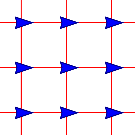
\includegraphics[scale=1]{figs/squarelattice}
        \end{figure}
      \end{column}%
    \end{columns}
\end{frame}

\begin{frame}{Lattice Graph}
  %\hrule
  %\begin{bclogo}[noborder=true, logo=\bccrayon]{} 
  \begin{block}{}
    \small{Given a lattice graph $G=(V, E)$ and a set of robots $R = \{
    r_1, \ldots, r_n \}$, $R$ \textbf{satisfies} $G$ if
    there exists a role function $f: R \rightarrow V$ that preserves
    the neighborhood structure of $G$.
    \\
    Specifically, for any $i$ and $j$, if $r_i$ and $r_j$ are neighbors, 
    there must exist an edge
    $e_{ij}: \edge{f(r_i)}{}{f(r_j)}$ in $E$, such that
    $ T(r_j) = T(r_i) T(e_{ij})$}
  %\end{bclogo}
  %\hrule 
  \begin{columns}[T] 
    \begin{column}{.4\textwidth}
      \begin{figure}
        \centering
        
\includegraphics[scale=0.38]{figs/hex}
      \end{figure}
    \end{column}%
    \begin{column}{.5\textwidth}
      \begin{figure}
        \centering
        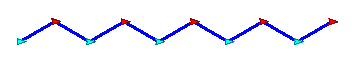
\includegraphics[width=\linewidth]{figs/bad-hexagon}
      \end{figure}
      \begin{figure}
        \centering
        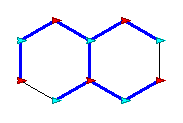
\includegraphics[scale=1]{figs/good-hexagon}
        \end{figure}
    \end{column}%
  \end{columns}
\end{block}
\end{frame}


\subsection{Algorithm}
\begin{frame}{Algorithm}
  \begin{block}{Robot broadcast message containing
      \textcolor{red}{authority} and \textcolor{red}{matching}}.
  \begin{columns}[T] % align columns
   \begin{column}{.5\textwidth}
      \begin{enumerate}
      \item Decides whether to be a \textcolor{red}{root}
        robot or a \textcolor{blue}{descendant} robot based on ``authority''
      \item Chooses a \textcolor{purple}{role} in the
        lattice graph. 
        % \begin{itemize}
        % \item \textcolor{red}{Root} robots always select the
        %   first lattice vertex as their role.  
        % \item \textcolor{blue}{Descendant} robots accept
        %   their roles as from their parents.
        % \end{itemize}    
      \item Computes a local task assignment for
        its neighbors and broadcasts this assignment to its neighbors.  
      \item Move to the destination. %Each \textcolor{blue}{descendant} robot moves toward to
        %the destination computed according to the assignment of its parent.
      \end{enumerate}
    \end{column}%
    \begin{column}{.5\textwidth}
      \begin{animateinline}[
        begin={%
          \begin{tikzpicture}%
           [post/.style={->,>=stealth', thin, draw=blue!50},
            node/.style={circle,fill=red!20,draw,font=\sffamily\small}]%
            \useasboundingbox (0,0) rectangle (5,5);
          },
          end={\end{tikzpicture}}
        ]{10}
         %\draw[dotted, violet, fill=violet!10] (3, 3) circle (3.5);
         \draw[fill=blue!50] (3,3) -- (2.75,3) -- (3.25,3.25) -- (3,2.75)  -- cycle;
         % \node[color=black] at (3, 4.5) {broadcast Message};           
         \draw[fill=blue!50] (0.5,4.5) -- (0.33,4) -- (0.5,4.125) -- (0.67,4) -- cycle;
         \draw[fill=blue!50] (1,1.5) -- (1.25,1) -- (1.25,1.25) --
         (1.5,1.25) -- cycle;
         \newframe*
         \multiframe{10}{rP = 0.1 +.1, r = 1 + 1}{ 
           \draw[fill=blue!50] (3,3) -- (2.75,3) -- (3.25,3.25) -- (3,2.75)  -- cycle;
           \node[color=black] at (3, 4.5) {broadcast Message};           
           \draw[fill=blue!50] (0.5,4.5) -- (0.33,4) -- (0.5,4.125) -- (0.67,4) -- cycle;
           \draw[fill=blue!50] (1,1.5) -- (1.25,1) -- (1.25,1.25) --
           (1.5,1.25) -- cycle;
           \path (3,3) -- (1.25, 1.25) node[pos=\rP] (q){};
           \draw[post] (3,3) -- (q.west);
           
           \path (3,3) -- (0.5, 4.125) node[pos=\rP] (q){};
           \draw[post] (3,3) -- (q.west);
           
           \path (1.5, 1.25) -- (3,2.5) node[pos=\rP] (q){};
           \draw[post] (1.5, 1.25) -- (q.west);
           
           \path (1.25, 1.5) -- (0.5, 4.125) node[pos=\rP] (q){};
           \draw[post] (1.25, 1.5) -- (q.south);
           
           \path (0.5, 4.5) -- (3.25, 3.25) node[pos=\rP] (q){};
           \draw[post] (0.5, 4.5) -- (q.north);

           \path (0.33, 4) -- (1, 1.5) node[pos=\rP] (q){};
           \draw[post] (0.33, 4) -- (q.north);
        }
        \newframe*
        \multiframe{10}{r = 1 + 1}{ 
         \draw[fill=red] (3,3) -- (2.75,3) -- (3.25,3.25) -- (3,2.75)  -- cycle;
         \node[color=red] at (3, 2.3) {$root$};           
         \draw[fill=blue] (0.5,4.5) -- (0.33,4) -- (0.5,4.125) --
         (0.67,4) 	-- cycle;
         \node[color=blue] at (1, 3.75) {$descendant$};           
         \draw[fill=blue] (1,1.5) -- (1.25,1) -- (1.25,1.25) -- (1.5,1.25)  -- cycle;
         \node[color=blue] at (2.5,1.5) {$descendant$};
         \node[color=black] at (3, 4.5) {Build Authority Tree};           
        }
        \newframe*
        \multiframe{10}{r = 1 + 1}{ 
          \draw[fill=red] (3,3) -- (2.75,3) -- (3.25,3.25) -- (3,2.75)  -- cycle;
         \node[color=red] at (3, 2.3) {$role:0$};           
         \draw[fill=blue] (0.5,4.5) -- (0.33,4) -- (0.5,4.125) --
         (0.67,4) 	-- cycle;
         \node[color=blue] at (1, 3.75) {$role:1$};           
         \draw[fill=blue] (1,1.5) -- (1.25,1) -- (1.25,1.25) -- (1.5,1.25)  -- cycle;
         \node[color=blue] at (2,1.5) {$role:2$};
         \node[color=black] at (3, 4.5) {Choose Role};           
        }
        \newframe*
        \multiframe{10}{r = 1 + 1}{ 
          \draw[fill=red] (3,3) -- (2.75,3) -- (3.25,3.25) -- (3,2.75)  -- cycle;
        % \node[color=red] at (3, 2.3) {$role:0$};           
         \draw[fill=blue] (0.5,4.5) -- (0.33,4) -- (0.5,4.125) --
         (0.67,4) 	-- cycle;
         %\node[color=blue] at (1, 3.75) {$role:1$};           
         \draw[fill=blue] (1,1.5) -- (1.25,1) -- (1.25,1.25) -- (1.5,1.25)  -- cycle;
         %\node[color=blue] at (3,1.5) {$role:2$};
         \node[color=black] at (3, 4.5) {Assign Task};  

         \draw[fill=red!40, dotted] (1,3) -- (0.75,3) -- (1.25,3.25) -- (1,2.75) -- cycle;
         \draw[fill=red!40, dotted] (3,1) -- (2.75,1) -- (3.25,1.25) -- (3,0.75) -- cycle;
         \draw[dashed](1.25,1.25) -- (3,1);
         \draw[dashed](0.5,4.125) -- (1,3);
        }
        \newframe*
        \multiframe{10}{r = 1 + 1}{ 
          \draw[fill=red] (3,3) -- (2.75,3) -- (3.25,3.25) -- (3,2.75)  -- cycle;
          \node[color=black] at (3, 4.5) {Move to Destination};  
          \draw[fill=blue] (1,3) -- (0.75,3) -- (1.25,3.25) -- (1,2.75) -- cycle;
          \draw[fill=blue] (3,1) -- (2.75,1) -- (3.25,1.25) -- (3,0.75) -- cycle;
       }
      \end{animateinline}
    \end{column}%
  \end{columns}
\end{block}
\end{frame}
%%%%%%%%%%%%%%%%
\subsection{Robot Authority}
\begin{frame}{Authority}
  \begin{bclogo}[logo=\bccrayon,couleur=orange!10, arrondi=0.2,
    ombre=true]{Definition}
    An \textbf{authority} is an ordered list of robot IDs
    $$(\id_1, \ldots, \id_k) $$
    The first ID in the list, $\id_1$ is called the \textbf{root} ID.
    Likewise, the final ID in the list, $\id_k$ is called the
    \textbf{sender} ID.  The number of IDs in the list is called
    its \textbf{length}.
  \end{bclogo}
  \begin{block}{Define a comparison operator for authorities}
    Authority $A_2$ is \textbf{higher than} $A_1$ if:
    \begin{itemize}
    \item \small{root ID of $A_2 >$ root ID of $A_1$, or}
    \item \small{length of $A_2 <$  length of $A_1$ if they have the same root, or}
    \item \small{sender ID of $A_2 >$ sender ID of $A_1$ if they have the same
    root and length }
  \end{itemize}

       
  \end{block}
\end{frame}

%%%%%%%%%%%%%%%%

% help me iron out the bugs or give me some comment and suggestions
\begin{frame}{Construct Authority Tree}{1. Decide to be root or descendant}
  \begin{block}{The robots use these authorities to establish a
      collection of authority trees}
    \begin{enumerate}
    \item Discards any message in which the authority contains its
      own ID.
    \item Forms an authority containing only its own ID,
      compares it with the authorities of remaining messages and
      selects the highest authority.
    \end{enumerate} 
  \begin{columns}[T] % align columns
    \begin{column}{.45\textwidth}
      \begin{itemize}
      \item If its authority is the highest, then it is
        the \textcolor{red}{root};
      \item Otherwise, it selects the one who sends the highest
        authority as its parent. Append its own ID to the highest
        authority to create its own authority. 
      \end{itemize}     
    \end{column}%
    \begin{column}{.45\textwidth}
       \begin{animateinline}[
        begin={%
          \begin{tikzpicture}%
           [post/.style={->,>=stealth', thick, draw=blue!50},
            node/.style={circle,fill=red!20,draw,font=\sffamily\small}]%
            \useasboundingbox (0,1) rectangle (5,5);
          },
          end={\end{tikzpicture}}
        ]{10}
        \draw[dashed, blue] (3, 4) circle (3);
        % center is (3,4)
        \draw[fill=blue!50] (3,4) -- (2.75,4) -- (3.25,4.25) -- (3,3.75)  -- cycle;
        \node[color=blue] at (2.75, 3.5) {$(2)$};
        % center is (0.5, 4.5)
        \draw[dashed, green] (0.5,4.5) circle (2.8);
        \draw[fill=green!50] (0.5,4.5) -- (0.33,4) -- (0.5,4.125) --
        (0.67,4) -- cycle;
        \node[color=green] at (0.5, 3.75) {$(4)$};
        % center is (3.75,2)
        \draw[dashed, red] (3.75,2) circle (2.5);
         \draw[fill=red!50] (3.5,2.5) -- (3.75,2) -- (3.75,2.25) --
         (4,2.25) -- cycle;
         \node[color=red] at (3.3, 2) {$(3)$};
         %%%%
        \newframe*
        \multiframe{10}{r = 1 + 1}{ 
          \draw[dashed, blue] (3, 4) circle (3);
          % center is (3,4)
          \draw[fill=blue!50] (3,4) -- (2.75,4) -- (3.25,4.25) --
          (3,3.75)  -- cycle;
          \node[color=blue] at (2.75, 3.5) {$(4,2)$};
          % center is (0.5, 4.5)
          \draw[dashed, green] (0.5,4.5) circle (2.8);
          \draw[fill=green!50] (0.5,4.5) -- (0.33,4) -- (0.5,4.125) --
          (0.67,4) -- cycle;
          \node[color=green] at (0.5, 3.75) {$(4)$};
          % center is (3.75,2)
          \draw[dashed, red] (3.75,2) circle (2.5);
          \draw[fill=red!50] (3.5,2.5) -- (3.75,2) -- (3.75,2.25) --
          (4,2.25) -- cycle;
          \node[color=red] at (3.3, 2) {$(3)$};
        }
        \newframe*
        \multiframe{10}{r = 1 + 1}{ 
          \draw[dashed, blue] (3, 4) circle (3);
          % center is (3,4)
          \draw[fill=blue!50] (3,4) -- (2.75,4) -- (3.25,4.25) --
          (3,3.75)  -- cycle;
          \node[color=blue] at (2.75, 3.5) {$(4,2)$};
          % center is (0.5, 4.5)
          \draw[dashed, green] (0.5,4.5) circle (2.8);
          \draw[fill=green!50] (0.5,4.5) -- (0.33,4) -- (0.5,4.125) --
          (0.67,4) -- cycle;
          \node[color=green] at (0.5, 3.75) {$(4)$};
          % center is (3.75,2)
          \draw[dashed, red] (3.75,2) circle (2.5);
          \draw[fill=red!50] (3.5,2.5) -- (3.75,2) -- (3.75,2.25) --
          (4,2.25) -- cycle;
          \node[color=red] at (3, 2) {$(4,2,3)$};
        }
         \newframe*
         \multiframe{10}{rP = 0.1 +.1, r = 1 + 1}{ 
           \draw[dashed, blue] (3, 4) circle (3);
          % center is (3,4)
          \draw[fill=blue!50] (3,4) -- (2.75,4) -- (3.25,4.25) --
          (3,3.75)  -- cycle;
          \node[color=blue] at (2.75, 3.5) {$(4,2)$};
          % center is (0.5, 4.5)
          \draw[dashed, green] (0.5,4.5) circle (2.8);
          \draw[fill=green!50] (0.5,4.5) -- (0.33,4) -- (0.5,4.125) --
          (0.67,4) -- cycle;
          \node[color=green] at (0.5, 3.75) {$(4)$};
          % center is (3.75,2.25)
          \draw[dashed, red] (3.75,2.25) circle (2.5);
          \draw[fill=red!50] (3.5,2.5) -- (3.75,2) -- (3.75,2.25) --
          (4,2.25) -- cycle;
          \node[color=red] at (3, 2) {$(4,2,3)$};
           \path (0.5,4.5) -- (3,4) node[pos=\rP] (q){};
           \draw[post] (0.5,4.125) -- (q.west);
           
           \path (3,4) -- (3.875, 2.25) node[pos=\rP] (q){};
           \draw[post] (3,4) -- (q.west);        
        }
      \end{animateinline}
    \end{column}
  \end{columns}
\end{block}
\end{frame}
%%%%%%%%%%%%%%%%

\begin{frame}{Construct Matching}{2. Role selection}
 \begin{block}{}
  Given a robot $r_i$ and a role vertex $v_i$ for that
  robot, let the lattice graph edge set $L=\{\emptyset,e_{ij}, e_{ik},
  \ldots\}$ be the set that contains a null value $\emptyset$ and all
  outgoing edges from vertex $v_i$. Let $Q=\{\id(r_a), \id(r_b),
  \ldots \}$ be the 
  \begin{columns}[T] % align columns
    \hspace{4mm}
    \begin{column}{.45\textwidth}
      set that contains the IDs of the neighbors of $r_i$.  
      \vspace{2mm}
      \hrule
      \hrule
     \begin{bclogo}[noborder=true, logo=\bccrayon]{} 
        A \textbf{matching} for a robot is a function $\eta : Q \rightarrow L$ that
        associates each neighbor ID with either a lattice graph edge
        from its role vertex or with the null value $\emptyset$.
      \end{bclogo}
      \hrule
      \hrule
    \end{column}%
    \begin{column}{.55\textwidth}
      \begin{figure}
        \centering
        \begin{tikzpicture}[
          fsnode/.style={},
          ssnode/.style={},
          every fit/.style={ellipse,draw,inner sep=0pt,text width=1cm},
          ->,shorten >= 2pt,shorten <= 2pt
          ]
          % the vertices of Q
          \begin{scope}[start chain=going below,node distance=1mm]
            \foreach \i/\xcoord in {1/\id(r_a),2/\id(r_b),3/\vdots, 4/\id(r_c)}
            \node[fsnode,on chain] (f\i) {$\xcoord$};
          \end{scope}
          % the vertices of L
          \begin{scope}[xshift=3cm,start chain=going below,node distance=1mm]
            \foreach \i/\xcoord in {5/e_{ij},6/e_{ik}, 7/\vdots, 8/\emptyset}
            \node[ssnode,on chain] (s\i) {$\xcoord$};
          \end{scope}         
          % the set U
          \node [myblue,fit=(f1) (f4),label=below:$Q$] {};
          % the set V
          \node [mygreen,fit=(s5) (s8),label=below:$L$] {};
          % the edges
          \draw (f1) -- (s6);
          \draw (f2) -- (s5);
          \draw (f4) -- (s8);
        \end{tikzpicture}
      \end{figure}
    \end{column}%
  \end{columns}
  \end{block}
\end{frame}
%%%%%%%%%%%%%%%%

% installation on Microsoft Windows Cont'd
\begin{frame}{Local Task Assignment}{3. Hungarain Algorithm}
  To compute an optimal matching of a robot with $N$ neighbors and $E$
  out-going edges of its role in the lattice graph, define a weight
  matrix of size $N \times \max(N, E)$ and apply
  \textcolor{scred}{Hungarian Algorithm}.
    \begin{columns}[T] % align columns
      \begin{column}{.5\textwidth}
        \begin{enumerate}
        \item Each row corresponds to a neighbor;
        \item Each column corresponds to an out-going edge of robot's
          role or a null value $\emptyset$.
        \item The entries of the matrix are the Euclidean distance
          between current position of each neighbor and the desired
          position if matched with a lattice graph edge.
        \end{enumerate}
      \end{column}%
      \begin{column}{.45\textwidth}
        \vspace{3mm}
           \begin{animateinline}[
             begin={%
               \begin{tikzpicture}%
                 [post/.style={->,>=stealth', thin, draw=blue!50},
                 node/.style={circle,fill=red!20,draw,font=\sffamily\small},
                 scale=0.7]%
                 %\useasboundingbox (0,0) rectangle (5,5);
               },
               end={\end{tikzpicture}}
             ]{10}
             \draw[fill=red] (3,3) -- (2.75,3) -- (3.25,3.25) -- (3,2.75) -- cycle;
             \draw[fill=blue!50] (0.5,4.5) -- (0.33,4) -- (0.5,4.125)
            -- (0.67,4) -- cycle;
            \draw[fill=blue!50] (4,5) -- (3.75,5.5) -- (3.75,5.25) -- (3.5,5.25)   	-- cycle;
            \draw[fill=blue!50] (1,2.5) -- (1.25,2) -- (1.25,2.25) -- (1.5,2.25)   	-- cycle;
            \draw[fill=blue!50] (5,2.92) -- (4.5,2.75) -- (5,2.58) -- (4.875,2.75)  -- cycle;
            \draw[fill=blue!50] (-0.5,2.5) -- (-0.5,2.75) -- (-0.75,2.25) -- (-0.25,2.5)  -- cycle;
            \draw[color=red] (4,4) -- (3.75,4) -- (4.25,4.25) -- (4,3.75) -- cycle;
            \draw[color=red] (2,2) -- (1.75,2) -- (2.25,2.25) -- (2,1.75) -- cycle;
            \draw[color=red] (2,4) -- (1.75,4) -- (2.25,4.25) -- (2,3.75) -- cycle;
            \draw[color=red] (4,2) -- (3.75,2) -- (4.25,2.25) -- (4,1.75) -- cycle;
             \newframe*
             \multiframe{10}{r = 1 + 1}{ 
              \draw[fill=red] (3,3) -- (2.75,3) -- (3.25,3.25) -- (3,2.75)   	-- cycle;
            \draw[fill=blue!50] (0.5,4.5) -- (0.33,4) -- (0.5,4.125) -- (0.67,4) 	-- cycle;
            \draw[fill=blue!50] (4,5) -- (3.75,5.5) -- (3.75,5.25) -- (3.5,5.25)   	-- cycle;
            \draw[fill=blue!50] (1,2.5) -- (1.25,2) -- (1.25,2.25) -- (1.5,2.25)   	-- cycle;
            \draw[fill=blue!50] (5,2.92) -- (4.5,2.75) -- (5,2.58) -- (4.875,2.75)  -- cycle;
            \draw[fill=blue!50] (-0.5,2.5) -- (-0.5,2.75) -- (-0.75,2.25) -- (-0.25,2.5)  -- cycle;
                        
            \draw[color=red] (4,4) -- (3.75,4) -- (4.25,4.25) -- (4,3.75) -- cycle;
            \draw[color=red] (2,2) -- (1.75,2) -- (2.25,2.25) -- (2,1.75) -- cycle;
            \draw[color=red] (2,4) -- (1.75,4) -- (2.25,4.25) -- (2,3.75) -- cycle;
            \draw[color=red] (4,2) -- (3.75,2) -- (4.25,2.25) -- (4,1.75) -- cycle;
            
            \draw[dashed](0.5, 4.25) -- (2,4);
            \draw[dashed](1.25,2.25) -- (2,2);
            \draw[dashed](3.75,5.25) -- (4,4);
            \draw[dashed](4.75,2.75) -- (4,2);
          }
        \end{animateinline}
        \vspace{3mm}
        \begin{flushleft}
          \footnotesize{A robot in red has 5 neighbors, its role in the lattice
           graph has 4 out-going edges. Use Hungarian algorithm to
           find the optimal matching for its neighbors.}
        \end{flushleft}
        
      \end{column}%
    \end{columns}
\end{frame}
%%%%%%%%%%%%%%%%

\begin{frame}{Robot Moving Strategy}{4. Robot Motion}
  % Define block styles
\tikzstyle{decision} = [diamond, draw, fill=red!10, 
    text width=4em, text badly centered, node distance=3cm, inner sep=0pt]
\tikzstyle{block} = [rectangle, draw, fill=blue!10, 
    text width=5em, text centered, rounded corners]%, minimum height=2em]
\tikzstyle{line} = [draw, -latex']

\begin{figure}    
\centering
\begin{tikzpicture}
    % Place nodes
    \node [block] (init) {\footnotesize{Start}};
    \node [decision, below of=init, node distance=2cm] (decide) {\footnotesize{Is root robot?}};
    \node [block, below of=decide, node distance=2cm] (root) {\footnotesize{Root}};
    \node [block, below of=root, node distance=2cm] (stop) {\footnotesize{Stay}};
    \node [block, right of=decide, node distance=3cm] (descendant) {\footnotesize{Descendant}};
    \node [decision, below of=descendant, node distance=2cm] (decideagain) {\footnotesize{Has
        matching?}};
    \node [block, right of=decideagain, node distance=3.5cm, text width=7em] (away)
    {\footnotesize{Move Away from its parent}};
    \node [block, below of=decideagain, node distance=2cm, text width=7em] (go)
    {\footnotesize{Move towards destination}};
    % Draw edges
    \path [line] (init) -- (decide);
    \path [line] (decide) -- node {yes}(root);
    \path [line] (root) -- (stop);
    \path [line] (decide) -- node {no} (descendant);
    \path [line] (descendant) -- (decideagain);
    \path [line] (decideagain) -- node {no} (away);
    \path [line] (decideagain) -- node {yes} (go);
  \end{tikzpicture}
  \end{figure}
\end{frame}
%%%%%%%%%%%%%%%%
\begin{frame}{Bounded Movement}{}
    \begin{columns}[T] % align columns
      \begin{column}{.5\textwidth}
        \begin{itemize}
        \item Set $O$ (\textcolor{red}{Red circle}) denotes the parent's
          observation at next stage.
        \item Descendant can be anywhere in set $P$ (\textcolor{blue}{blue
            circle}) at next stage.
        \item The real destination for descendant is the closest
          position on the boundary of the intersection ($O\cap P$) to
          the assigned destination.
        \end{itemize}
      \end{column}%
      \begin{column}{.5\textwidth}
      % Definition of circles
        \def\firstcircle{(0,0) circle (2cm)}
        \def\secondcircle{(2.3,1.8) circle (1.5cm)}
        \def\thirdcircle{(0,0) circle (1.5cm)}
        \colorlet{circle edge}{blue!50}
        \colorlet{circle area}{blue!20}
        \tikzset{filled/.style={fill=circle area, draw=circle edge, thick},
          outline/.style={draw=circle edge, thick}}
        \tikzstyle{important line}=[very thick]
        % Set A and B
        \begin{tikzpicture}[scale=0.65]
          \begin{scope}
            \clip \firstcircle;
            \fill[filled] \secondcircle;
          \end{scope}       
          \draw[outline, red] \firstcircle node {$ $}; 
          \draw[fill=circle area, red] (0,0) circle (0.1cm); 
          \node at (-0.75,-0.3) {Parent};
          
          \draw[outline]
          \secondcircle node {$ $};

          \draw[fill=circle area, blue] (2.3,1.8) circle (0.1cm); 
          \node at (3.2, 2.3) {Descendant};

          \draw[fill=circle area, blue] (3, -0.7) circle (0.1cm); 
          \node at (3.8,-1) {Assigned Destination};

          \draw[fill=circle area, blue] (1.96, 0.32) circle (0.1cm); 
          \node  at (3.5,0) {Real Destination};
        \end{tikzpicture}
      \end{column}%
    \end{columns}
\end{frame}
%%%%%%%%%%%%%%%%


\section{Results}
\begin{frame}{Simulation}{Octagon-square formation with 100 robots}
  \begin{center}
    \includemovie[toolbar,poster,autoplay]{7cm}{7cm}{octsq1000009v12sr55.mp4}
  \end{center}
\end{frame}
%%%%%%%%%%%%%%%%%%%%%%%%%%%%
\begin{frame}{Simulation}{Hexagon formation with 100 robots}
  \begin{center}
    \includemovie[toolbar,poster,autoplay]{7cm}{7cm}{hexagon1000009v12.mp4}
  \end{center}
\end{frame}
%%%%%%%%%%%%%%%%

\begin{frame}{Experiments}{on three kinds of repeated
    lattice patterns}
  \begin{block}{Experiments Setup}
    \begin{itemize}
    \item Varied the number of robots $n$.
    \item For each $n$, repeated the experiment $50$ times.
    \item Initially all robots are uniformly distributed in each experiment.
    \end{itemize}
  \end{block}
  
    \begin{columns}
      \begin{column}{.6\textwidth}
        \begin{block}{Measurements}
          \begin{itemize}
          \item Average time to real static position
          \item Average non-fulfillment ratio: $\Gamma =
            \dfrac{1}{n}\sum\limits_{i=1}^n \frac{E_i - N_i}{E_i}$
          \end{itemize}
        \begin{figure}
          \centering
          %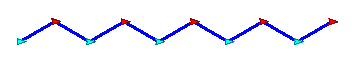
\includegraphics[width=\linewidth]{figs/bad-hexagon}
        \end{figure}
      \end{block}
      \end{column}
      \begin{column}{.3\textwidth}
        
      \end{column}
    \end{columns} 
\end{frame}

%%%%%%%%%%%%%%%%
% how to modify the theme
% {\setbeamercolor{AAUsimple}{fg=gray!50,bg=orange!50}
%  \setbeamercolor{structure}{fg=red}
%  \setbeamercolor{frametitle}{use=structure,fg=structure.fg}
%  \setbeamercolor{normal text}{bg=gray!20}
\begin{frame}{Results}{on three kinds of repeated
lattice patterns}
\textcolor{scred}{Average time and its standard deviation
            of forming repeated \\ 
            lattice patterns of square, hexagon
            and octagon-square}
          \begin{figure}
            \centering
            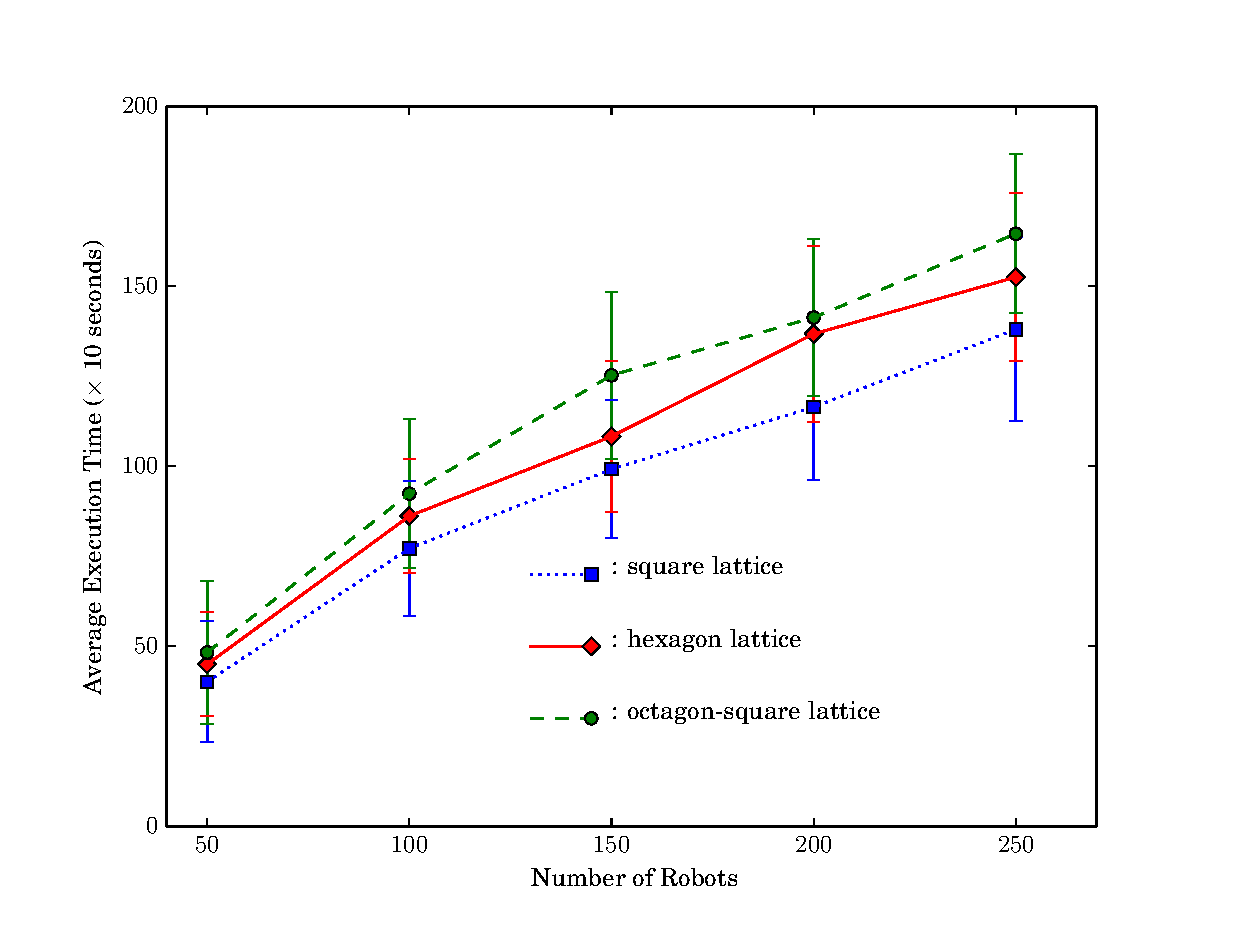
\includegraphics[width=0.75\textwidth]{figs/exptime}
          \end{figure}

\end{frame}
%%%%%%%%%%%%%%%%
\begin{frame}{Results}{on three kinds of repeated
lattice patterns}
\textcolor{scred}{Average non-fulfillment ratio and its standard
            deviation of forming\\ repeated
            lattice patterns of square, hexagon
            and octagon-square}
          \begin{figure}
            \centering
            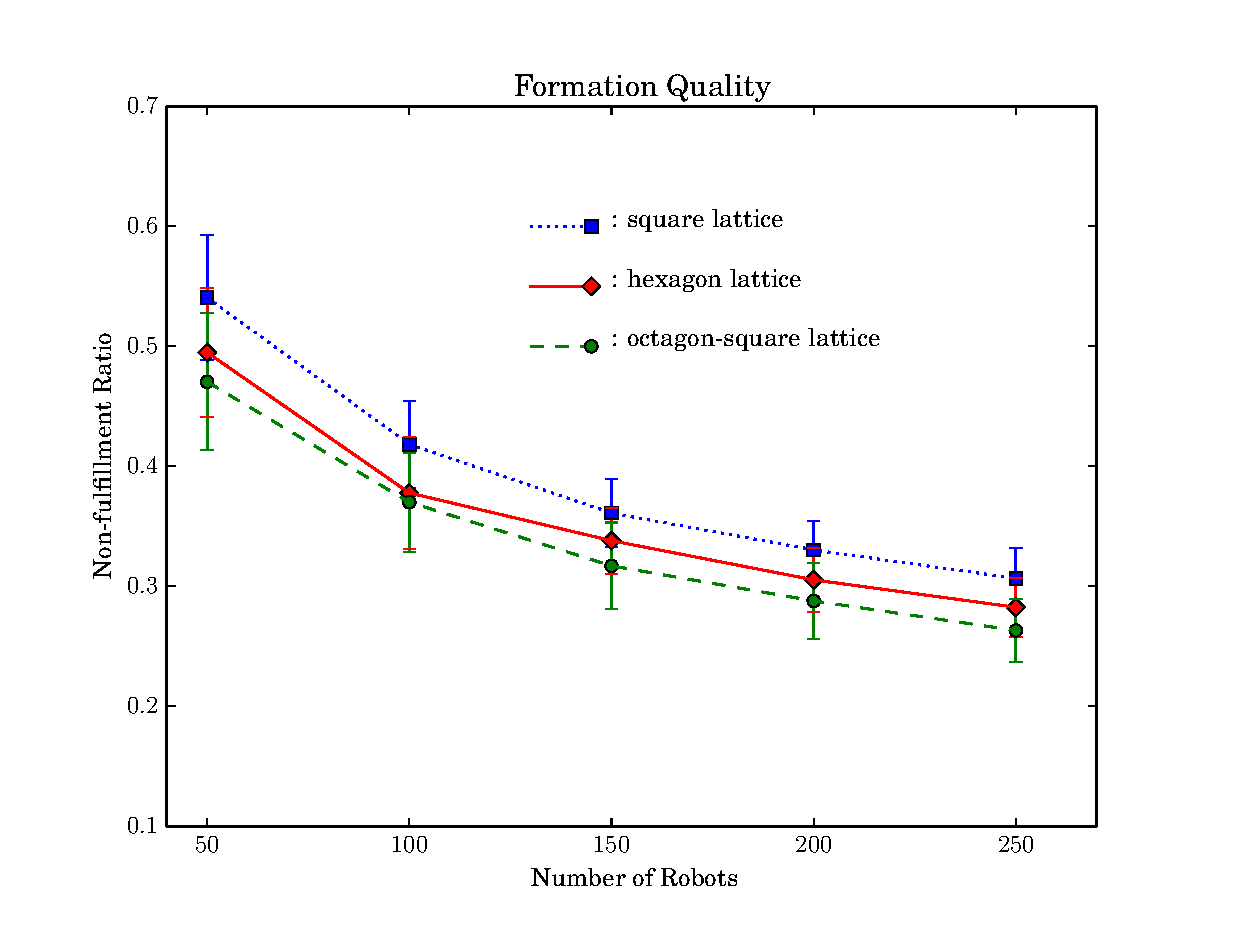
\includegraphics[width=0.75\textwidth]{figs/expqual}
          \end{figure}
\end{frame}

\subsection{Conclusions}
% Widescreen Support
\begin{frame}{Conclusions}{}
\begin{block}{Summary}
  \begin{itemize}
  \item Robots can form different types of geometric formations,
    including the repeated lattice patterns
  \item Algorithm scales reasonably well with increasing numbers of
    robot
  \item Algorithm is robust to the situation when some robots are removed from or
    with more robots added to the system
  \end{itemize}
\end{block}
\begin{block}{Future Work}
  \begin{itemize}
  \item Promote the motion strategy
  \item Theoretically prove the convergence of the algorithm 
  \item Extend the algorithm to the multi-robot systems subject to the nonholonomic
    constraints
  \end{itemize}
\end{block}
\end{frame}
%%%%%%%%%%%%%%%%


%\subsection{Questions}
% contact information
% \begin{frame}{Questions}{}
%   \begin{center}
%     \textcolor{scred}{\LARGE $\mathscr{THANK}$ $\mathscr{YOU}!$}
%   \end{center}
% \end{frame}
%%%%%%%%%%%%%%%%

\end{document}
